\documentclass{article}

\usepackage{float}
\usepackage{mathtools}
\usepackage{graphicx}
\usepackage{geometry}
\usepackage{subfig}
\usepackage[table]{xcolor}
\usepackage{bera}
\usepackage{listings}
\usepackage{xepersian}


\geometry{margin=20mm}

\settextfont{B Nazanin}

\graphicspath{ {./pics/} }

\definecolor{codegreen}{rgb}{0,0.6,0}
\definecolor{codegray}{rgb}{0.5,0.5,0.5}
\definecolor{codepurple}{rgb}{0.58,0,0.82}
\definecolor{backcolour}{rgb}{0.95,0.95,0.92}

\lstdefinestyle{mystyle}{
    backgroundcolor=\color{backcolour},   
    commentstyle=\color{codegreen},
    keywordstyle=\color{blue},
    numberstyle=\tiny\color{codegray},
    stringstyle=\color{codepurple},
    basicstyle=\ttfamily\footnotesize,
    breakatwhitespace=false,         
    breaklines=true,                 
    captionpos=b,                    
    keepspaces=true,                 
    numbers=left,                    
    numbersep=5pt,                  
    showspaces=false,                
    showstringspaces=false,
    showtabs=false,                  
    tabsize=2
}

\lstset{style=mystyle}


\begin{document}
\title{پروژه‌ی درس مقدمه‌ای بر رباتیک}

\date{خرداد ماه ۱۴۰۱}
\author{فروغ افخمی اردکانی، علی بهمنیار، سینا ربیعی، سمیرا سلجوقی}
\maketitle
\noindent
\section{بررسی مشخصات ربات}
\begin{figure}[H]%
    \centering
    \subfloat{{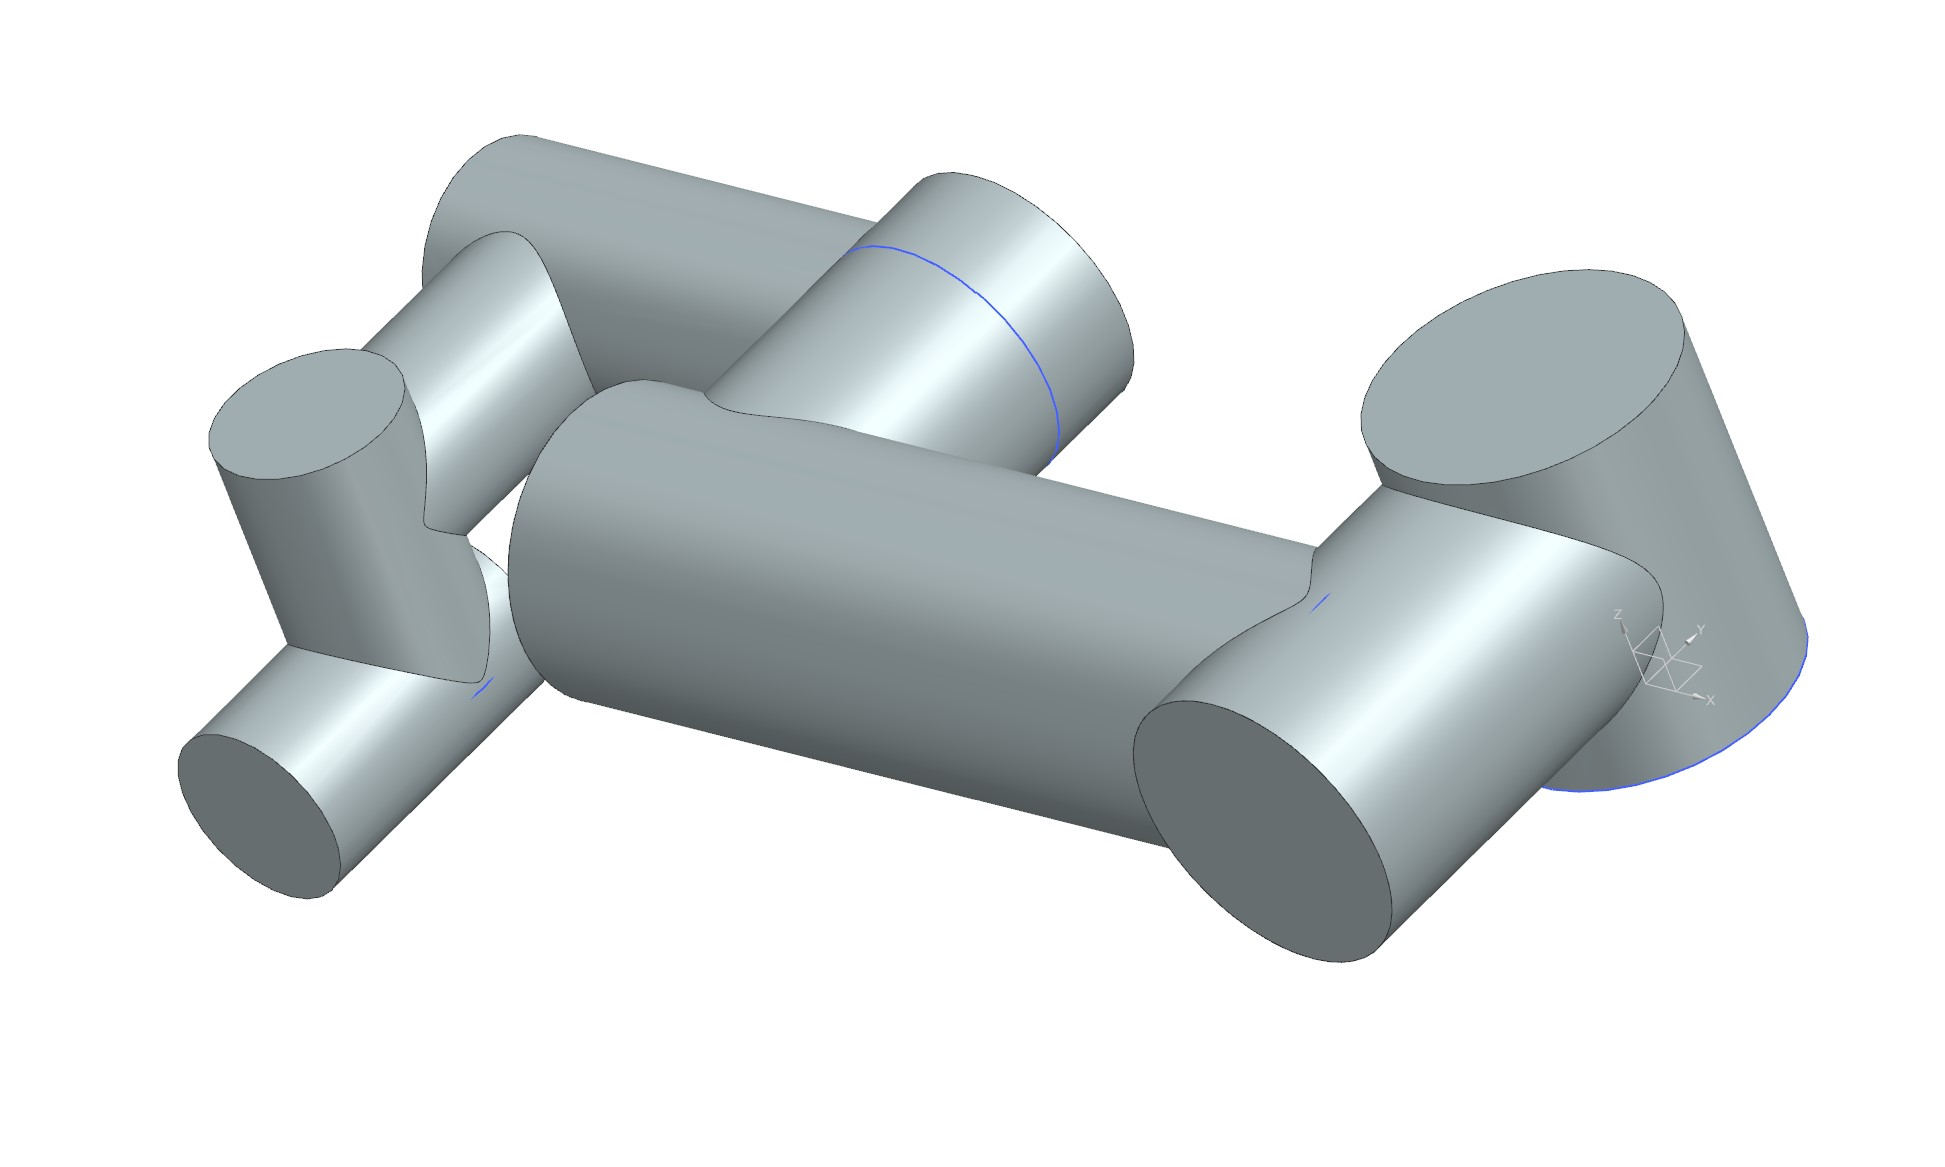
\includegraphics[height=6cm]{p1}}}
    \qquad
    \subfloat{{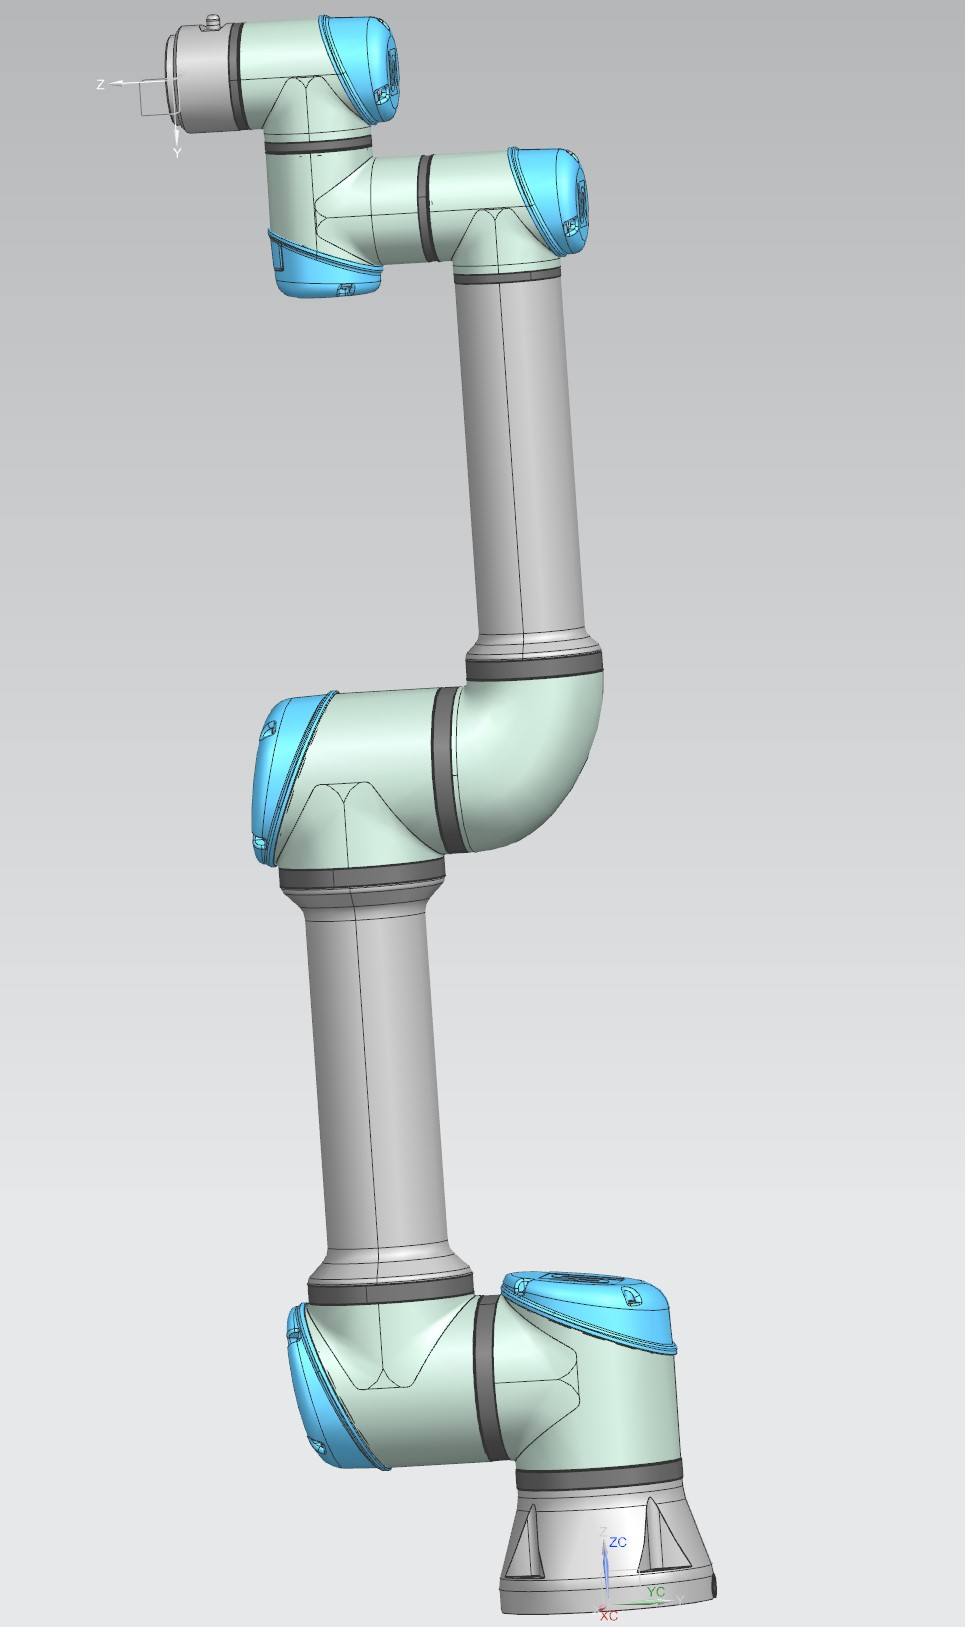
\includegraphics[height=6cm]{p2}}}
    \caption{طراحی مدل سه بعدی ربات در نرم افزار \lr{NX} و محاسبه‌ی مشخصات ربات از روی آن \label{fig:fig1}}
\end{figure}


\section{به دست آوردن پارامتر‌های دناویت-هارتنبرگ}
ابتدا با توجه به دناویت هارتنبرگ اصلاح شده \lr{(Modified)} فریم‌ها را به مفصل‌های ربات اختصاص می دهیم و سپس جدول مربوطه را تکمیل می کنیم:
\begin{figure}[H]%
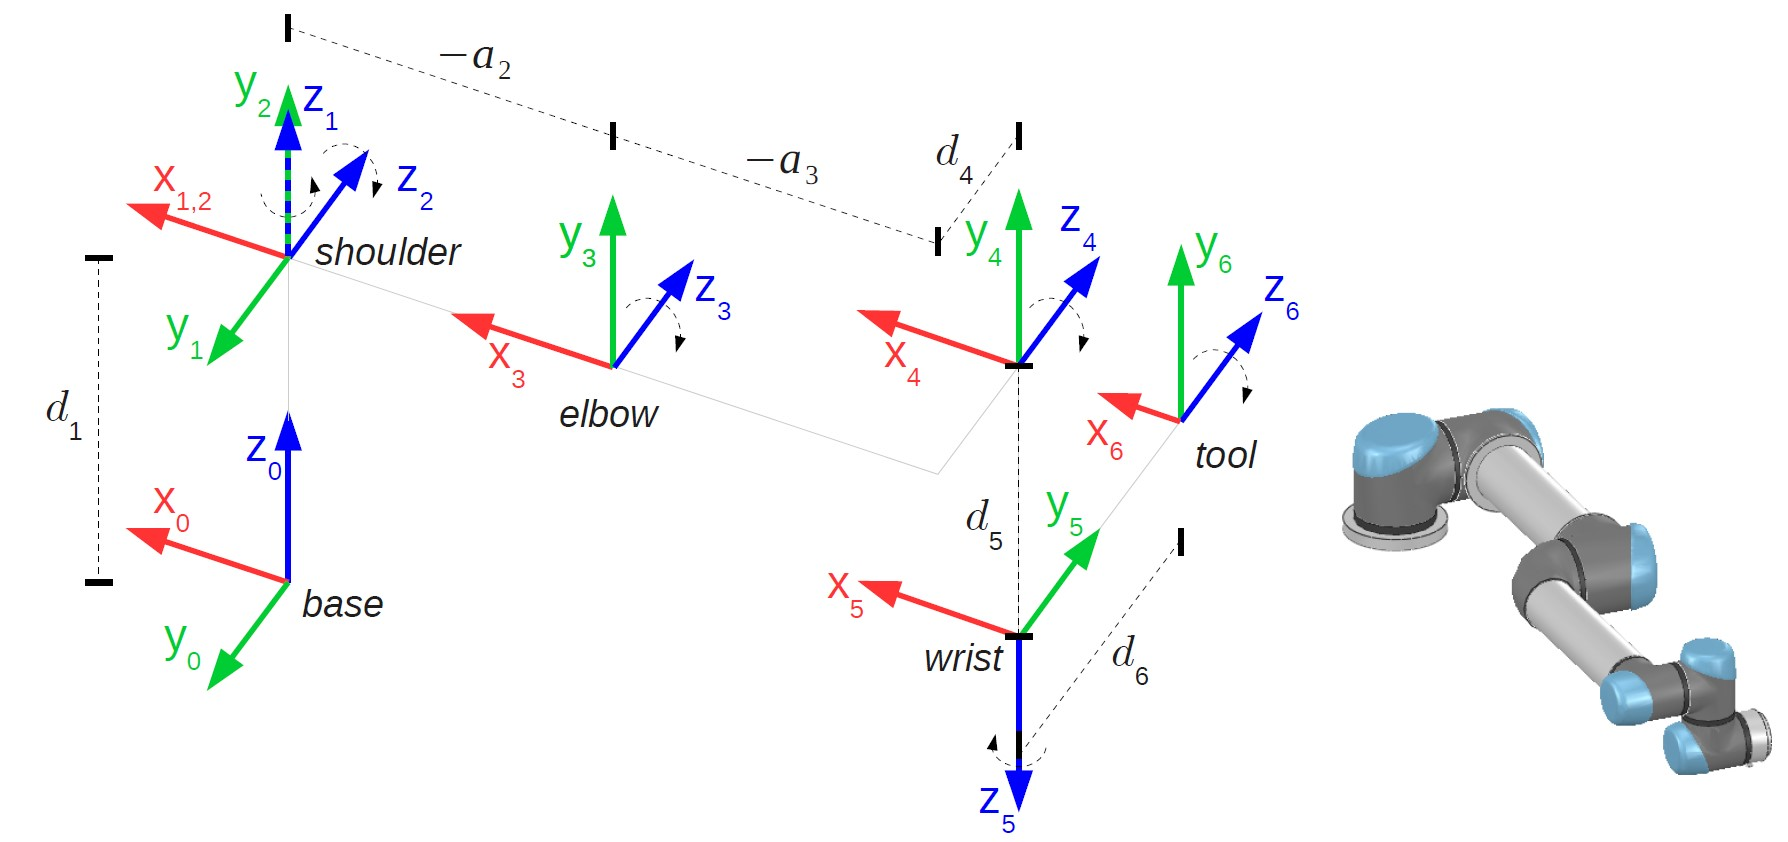
\includegraphics[height=6cm]{p3}
\label{fig:fig2}
\caption{قرارگیری محورهای دناویت-هارتنبرگ بر روی ربات}
\end{figure}




\begin{table}
\begin{latin}
\begin{center}
\begin{tabular}{ c | c c c c }
 $i$ & $a_{i-1}$ & $\alpha_{i-1}$ & $d_{i}$ & $\theta_{i}$ \\ 
 \hline
 1 & 0 & 0 & $d_{1}$ & $\theta_{1}$ \\  
 2 & 0 & 90 & $0$ & $\theta_{2}$ \\ 
 3 & $a_{2}$ & 0 & $0$ & $\theta_{3}$ \\ 
 4 & $a_{3}$ & 0 & $d_{4}$ & $\theta_{4}$ \\ 
 5 & 0 & 90 & $d_{5}$ & $\theta_{5}$ \\ 
 6 & 0 & -90 & $d_{6}$ & $\theta_{6}$
 
\end{tabular}
\end{center}
\end{latin}
\caption{پارامترهای دناویت-هارتنبرگ}
\label{table:1}
\end{table}
\begin{gather*}
Modified\ DH: \\
T_{1}^{0} = \begin{bmatrix}
C_{1} & -S_{1} & 0 & 0 \\
S_{1} & C_{1} & 0 & 0 \\
0 & 0 & 1 & d_{1} \\
0 & 0 & 0 & 1
\end{bmatrix}
\quad
T_{2}^{1} = \begin{bmatrix}
C_{2} & -S_{2} & 0 & 0 \\
0 & 0 & -1 & 0 \\
S_{2} & C_{2} & 0 & 0 \\
0 & 0 & 0 & 1
\end{bmatrix}
\quad
T_{3}^{2} = \begin{bmatrix}
C_{3} & -S_{3} & 0 & a_{2} \\
S_{3} & C_{3} & 0 & 0 \\
0 & 0 & 1 & 0 \\
0 & 0 & 0 & 1
\end{bmatrix}
\\
T_{4}^{3} = \begin{bmatrix}
c_{4} & -S_{4} & 0 & a_{3} \\
S_{4} & C_{4} & 0 & d_{4} \\
0 & 0 & 1 & 0 \\
0 & 0 & 0 & 1
\end{bmatrix}
\quad
T_{5}^{4} = \begin{bmatrix}
C_{5} & -S_{5} & 0 & 0 \\
0 & 0 & -1 & -d_{5} \\
S_{5} & C_{5} & 0 & 0 \\
0 & 0 & 0 & 1
\end{bmatrix}
\quad
T_{6}^{5} = \begin{bmatrix}
C_{6} & -S_{6} & 0 & 0 \\
0 & 0 & 1 & d_{6} \\
-S_{6} & -C_{6} & 0 & 0 \\
0 & 0 & 0 & 1
\end{bmatrix}
\end{gather*}
\section{به دست آوردن موقعیت مجری نهایی}
در ادامه در متلب تابعی با نام \lr{DH} تعریف می کنیم که متغیر های مفاصل را با بردار $t$ و پارامتر های ثابت ربات را به عنوان ورودی دریافت می‌کند و در خروجی با توجه به جدول  \lr{DH} ماتریس‌های تبدیل را خروجی می‌دهد.
\\
حال در فایل \lr{FK.m} این تابع را با تعریف متغیر‌های گفته شده صدا می‌زنیم و ماتریس‌های تبدیل را به دست می‌آوریم. در بخش صحت‌سنجی نیز در ابتدا مقادیر پارامتر‌های ثابت را که از دیتاشیت جمع آوری کرده بودیم، قرار می‌دهیم و حالت \lr{zero configuration} ربات را در نظر می‌گیریم.
سپس با استفاده از توابع  \lr{Peter Corke} ابتدا لینک‌های ربات را با دستور $Link$ با فرمت زیر تعریف می کنیم:
\begin{latin}
\begin{lstlisting}[language=matlab, caption=Peter Corke's Link, label=code:s1]
L = Link(dh, options)

DH = [THETA D A ALPHA SIGMA OFFSET]

% theta: joint angle
% d: link offset
% a: link length
% alpha: link twist
% sigma: 0 if revolute, 1 if prismatic
\end{lstlisting}
\end{latin}
\noindent
در ادامه با دستور $SerialLink$ لینک‌ها را به هم مرتبط می‌سازیم و در نهایت با دستور $fkine$ و دادن  \lr{zero configuration} در ورودی، ماتریس‌های تبدیل را به دست می آوریم که نتایج با نتایج بخش قبل یکسان است.
\\
برای ماتریس های دوران نیز ابتدا تابعی تعریف می کنیم \lr{(RDH.m)} که ماتریس‌های تبدیل را در ورودی دریافت کرده و با جدا کردن بخش دوران آن، ماتریس‌های دوران را خروجی می دهد و در نهایت با صدا زدن این تابع در فایل \lr{Rotation.m } ماتریس‌های دوران را به دست می آوریم:

\begin{latin}
%\lstinputlisting[language=matlab, caption=Matlab, label=code:m3_3]{codes/m3_3.m}
\end{latin}

\subsection{ماتریس $H$}
\scalebox{0.5}{
\begin{latin}
    $\displaystyle \begin{array}{l}
\left(\begin{array}{cccc}
\cos \left(t_6 \right)\,\sigma_5 -\sigma_1 \,\cos \left(t_1 \right)\,\sin \left(t_6 \right) & -\sin \left(t_6 \right)\,\sigma_5 -\sigma_1 \,\cos \left(t_1 \right)\,\cos \left(t_6 \right) & \sigma_3  & d_6 \,\sigma_3 +d_4 \,\sin \left(t_1 \right)-a_3 \,\cos \left(t_2 +t_3 \right)\,\cos \left(t_1 \right)-a_2 \,\cos \left(t_1 \right)\,\cos \left(t_2 \right)+d_5 \,\sigma_1 \,\cos \left(t_1 \right)\\
-\cos \left(t_6 \right)\,\sigma_4 -\sigma_1 \,\sin \left(t_1 \right)\,\sin \left(t_6 \right) & \sin \left(t_6 \right)\,\sigma_4 -\sigma_1 \,\cos \left(t_6 \right)\,\sin \left(t_1 \right) & -\sigma_2 -\sigma_6  & d_5 \,\sigma_1 \,\sin \left(t_1 \right)-d_4 \,\cos \left(t_1 \right)-a_3 \,\cos \left(t_2 +t_3 \right)\,\sin \left(t_1 \right)-a_2 \,\cos \left(t_2 \right)\,\sin \left(t_1 \right)-d_6 \,{\left(\sigma_2 +\sigma_6 \right)}\\
\sigma_7 \,\sin \left(t_6 \right)+\sigma_1 \,\cos \left(t_5 \right)\,\cos \left(t_6 \right) & \sigma_7 \,\cos \left(t_6 \right)-\sigma_1 \,\cos \left(t_5 \right)\,\sin \left(t_6 \right) & -\sigma_1 \,\sin \left(t_5 \right) & d_1 +d_5 \,{\left(\sin \left(t_2 +t_3 \right)\,\sin \left(t_4 \right)-\cos \left(t_2 +t_3 \right)\,\cos \left(t_4 \right)\right)}-a_3 \,\sin \left(t_2 +t_3 \right)-a_2 \,\sin \left(t_2 \right)-d_6 \,\sin \left(t_5 \right)\,{\left(\cos \left(t_2 +t_3 \right)\,\sin \left(t_4 \right)+\sin \left(t_2 +t_3 \right)\,\cos \left(t_4 \right)\right)}\\
0 & 0 & 0 & 1
\end{array}\right)\\
\mathrm{}\\
where
\mathrm{}\\
\;\;\sigma_1 =\sin \left(t_2 +t_3 +t_4 \right)\\
\mathrm{}\\
\;\;\sigma_2 =\cos \left(t_1 \right)\,\cos \left(t_5 \right)\\
\mathrm{}\\
\;\;\sigma_3 =\cos \left(t_5 \right)\,\sin \left(t_1 \right)-\sigma_7 \,\cos \left(t_1 \right)\,\sin \left(t_5 \right)\\
\mathrm{}\\
\;\;\sigma_4 =\cos \left(t_1 \right)\,\sin \left(t_5 \right)-\sigma_7 \,\cos \left(t_5 \right)\,\sin \left(t_1 \right)\\
\mathrm{}\\
\;\;\sigma_5 =\sin \left(t_1 \right)\,\sin \left(t_5 \right)+\sigma_7 \,\cos \left(t_1 \right)\,\cos \left(t_5 \right)\\
\mathrm{}\\
\;\;\sigma_6 =\sigma_7 \,\sin \left(t_1 \right)\,\sin \left(t_5 \right)\\
\mathrm{}\\
\;\;\sigma_7 =\cos \left(t_2 +t_3 +t_4 \right)
\end{array}$
\end{latin}
}

\subsection{ماتریس $R$}
\begin{latin}
    $\displaystyle \begin{array}{l}
\left(\begin{array}{ccc}
\cos \left(t_6 \right)\,\sigma_3 -\sigma_1 \,\cos \left(t_1 \right)\,\sin \left(t_6 \right) & -\sin \left(t_6 \right)\,\sigma_3 -\sigma_1 \,\cos \left(t_1 \right)\,\cos \left(t_6 \right) & \cos \left(t_5 \right)\,\sin \left(t_1 \right)-\sigma_4 \,\cos \left(t_1 \right)\,\sin \left(t_5 \right)\\
-\cos \left(t_6 \right)\,\sigma_2 -\sigma_1 \,\sin \left(t_1 \right)\,\sin \left(t_6 \right) & \sin \left(t_6 \right)\,\sigma_2 -\sigma_1 \,\cos \left(t_6 \right)\,\sin \left(t_1 \right) & -\cos \left(t_1 \right)\,\cos \left(t_5 \right)-\sigma_4 \,\sin \left(t_1 \right)\,\sin \left(t_5 \right)\\
\sigma_4 \,\sin \left(t_6 \right)+\sigma_1 \,\cos \left(t_5 \right)\,\cos \left(t_6 \right) & \sigma_4 \,\cos \left(t_6 \right)-\sigma_1 \,\cos \left(t_5 \right)\,\sin \left(t_6 \right) & -\sigma_1 \,\sin \left(t_5 \right)
\end{array}\right)\\
\mathrm{}\\
where\\
\mathrm{}\\
\;\;\sigma_1 =\sin \left(t_2 +t_3 +t_4 \right)\\
\mathrm{}\\
\;\;\sigma_2 =\cos \left(t_1 \right)\,\sin \left(t_5 \right)-\sigma_4 \,\cos \left(t_5 \right)\,\sin \left(t_1 \right)\\
\mathrm{}\\
\;\;\sigma_3 =\sin \left(t_1 \right)\,\sin \left(t_5 \right)+\sigma_4 \,\cos \left(t_1 \right)\,\cos \left(t_5 \right)\\
\mathrm{}\\
\;\;\sigma_4 =\cos \left(t_2 +t_3 +t_4 \right)
\end{array}$

\end{latin}

\section{به دست آوردن زوایای مجری نهایی}
در این بخش روابط مربوط به هر کدام از نمایش‌ها را از کتاب های مرجع استخراج می‌کنیم و با داشتن ماتریس‌های تبدیل این نمایش‌ها را برای مجری نهایی ربات بر حسب متغیر‌های مفصلی به دست می‌آوریم.
\subsection{نمایش محور-زاویه\lr{(Equivalent angle—axis representation)}:}
\begin{figure}[H]%
    \centering
    \subfloat{{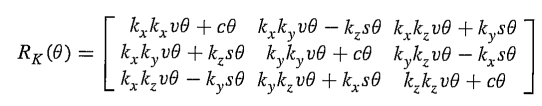
\includegraphics[height=2cm]{formulas/1}}}
    \qquad
    \subfloat{{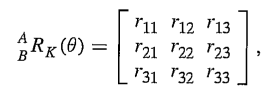
\includegraphics[height=2cm]{formulas/2}}}
    \qquad
    \subfloat{{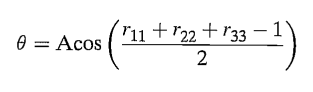
\includegraphics[height=2cm]{formulas/3}}}
    \qquad
    \subfloat{{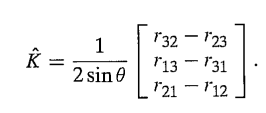
\includegraphics[height=2cm]{formulas/4}}}
    \caption{روابط نمایش محور-زاویه\label{fig:formula1}}
\end{figure}

\subsection{نمایش زوایای ثابت\lr{(X-Y-Z fixed angles)}:}
\begin{figure}[H]%
    \centering
    \subfloat{{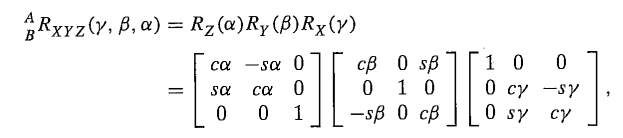
\includegraphics[height=2cm]{formulas/5}}}
    \qquad
    \subfloat{{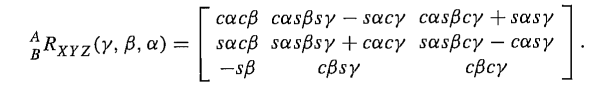
\includegraphics[height=2cm]{formulas/6}}}
    \qquad
    \subfloat{{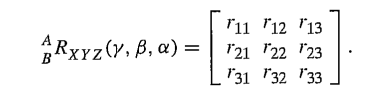
\includegraphics[height=2cm]{formulas/7}}}
    \qquad
    \subfloat{{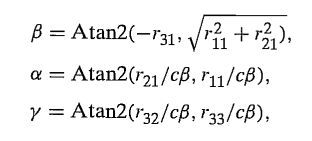
\includegraphics[height=2cm]{formulas/8}}}
    \caption{روابط نمایش زوایای ثابت\label{fig:formula2}}
\end{figure}

\subsection{نمایش زوایای اویلر\lr{(X-Y-Z Euler angles)}:}
\begin{figure}[H]%
    \centering
    \subfloat{{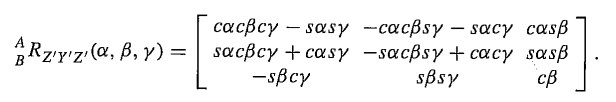
\includegraphics[height=2cm]{formulas/9}}}
    \qquad
    \subfloat{{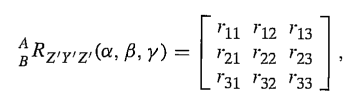
\includegraphics[height=2cm]{formulas/10}}}
    \qquad
    \subfloat{{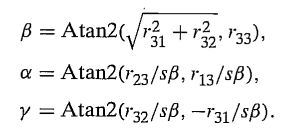
\includegraphics[height=2cm]{formulas/11}}}
    \caption{روابط نمایش زوایای اویلر\label{fig:formula3}}
\end{figure}


\subsection{نمایش چهارگانه یکه\lr{(Quaternion)}:}
\begin{latin}
\begin{gather*}
-1 = i^2 = j^2 = k^2 \\ i = jk = -kj\\ j = ki = -ik \\k = ij = -ji \\
Q = q_0 + iq_1 + jq_2 + kq_3 \quad q_0^2 + q_1^2 + q_2^2 + q_3^2 = 1 \\
\text{Rotation by $\theta$ about the unit vector $n = (n_x, n_y, n_z)^T$} \\
\downarrow \\
Q = (cos \frac{\theta}{2},n_x sin \frac{\theta}{2}, n_y sin \frac{\theta}{2},n_z sin \frac{\theta}{2})
\end{gather*}
\end{latin}

\section{به دست آوردن فضای کاری ربات}
برای به دست آوردن فضای کاری پس از تعیین کردن مقادیر ثابت ربات، یک حلقه تو در تو به تعداد درجات آزادی ربات (6) ایجاد می کنیم که هر حلقه یکی از متغیر‌های مفصلی را از صفر تا $2\pi$ با فواصل $0.07\pi$ می‌چرخاند (با کاهش فواصل دقت فضای کاری بیشتر و در نتیجه حجم اطلاعات و زمان اجرا شدن برنامه بیشتر خواهد شد).
\\
در ادامه در داخلی ترین حلقه، ماتریس تبدیل مجری نهایی به دستگاه پایه را به دست می‌آوریم و ماتریس‌های $x$ و $y$ و $z$ را که به ترتیب سه سطر اول ستون چهارم ماتریس تبدیل است را مشخص می کنیم. 
برای پر شدن ماتریس های $x$ و $y$ و $z$ در طی اجرا شدن حلقه، یک شمارنده \lr{(iterator)} به نام $b$ در خارج از حلقه‌ها تعریف می کنیم که در هر بار ماتریس‌های فوق را یک ستون جلو ببرد.
\\
در نهایت با ترانهاده کردن ماتریس های $x$ و $y$ و $z$ یک ماتریس $P$ تعریف می کنیم که ستون‌های آن مقادیر $x$ و $y$ و $z$ هستند و سپس با داشتن این ماتریس، دستور $trisurf$ مرز و محدوده خارجی این داده ها را رسم می کند که فضای کاری ربات را مشخص می کند. (تعداد همه‌ی نقاط فضای کاری بسیار زیاد است و رسم آن زمان خیلی زیادی می برد، به همین منظور فقط مرز آن را رسم میکنیم)
با توجه به اینکه ربات 6 درجه آزادی دارد و بنابر دیتاشیت آن هیچ کدام از مفاصل دورانی محدودیتی برای گردش ندارند، فضای کاری ربات یک کره خواهد شد؛ همانطور که در بالا توضیح داده شد، به دلیل اندازه‌ی $step$های استفاده شده در رسم نمودار شکل \ref{fig:ws}، شکل به دست آمده یک کره‌ی ایده‌آل نیست اما با کاهش $step$های رسم، شکل فضای کاری به کره نزدیک‌تر خواهد شد:
\begin{figure}[H]%
	\centering
	\includegraphics[height=6cm]{ws}
    \caption{فضای کاری ربات در فضای سه بعدی}
    \label{fig:ws}
\end{figure}
برای صحت سنجی این بخش نیز مشابه قسمت سینماتیک مستقیم ابتدا لینک‌ها را تعریف کرده و سپس با دستور $plot$ (مربوط به تولباکس \lr{Peter Corke}) و $pause$ در همان حلقه‌های تو در تو در هر بار فضای کاری را رسم می‌کنیم. آپشن‌های $‘jvec’$ و $‘noname’$ نیز فریم‌ها را بر روی ربات نمایش داده و همچنین اسم روی صفحه را پاک می‌کنند.

\section{سینماتیک معکوس ربات}
برای محاسبه سینماتیک معکوس تابعی به نام \lr{inverse} تعریف می کنیم که 6 ورودی شامل جهت گیری و موقعیت مجری نهایی ربات دارد و خروجی آن بردار پارامترهای مفصلی است.
در این تابع ابتدا پارامترهای ثابت ربات را مقدار دهی می کنیم و $x$ و $y$ و $z$ را \lr{concatante} میکنیم و در بردار $P60$ ($P_6^0$) قرار می‌دهیم.
سپس با استفاده از قاعده زوایای ثابت و جهت گیری مجری نهایی (داده شده در ورودی) ماتریس های دوران $x,y,z$ را به دست می‌آوریم و با ضرب این سه ماتریس در یک دیگر ماتریس دوران مجری نهایی را نسبت به فریم $0$ محاسبه میشود.
با کنار هم قرار دادن ماتریس $R60$ و بردار $P60$ و قرار دادن یک سطر \lr{dumy} ،ماتریس $T60$ به دست می‌آوریم.

\subsection{محاسبه‌ی $\theta_1$}
ابتدا یک مثلث تشکیل می‌دهیم که سه زاویه ان همان مراکز محور های فریم های $0,5,6$ میباشند. سپس با توجه به شکل میتوان دید که موقعیت مفصل 5 ام برابر است با موقعیت مفصل 6 ام منهای $d_6$ که $d_6$ در جهت $z_6$ میباشد.

\begin{figure}[H]%
    \centering
    \subfloat{{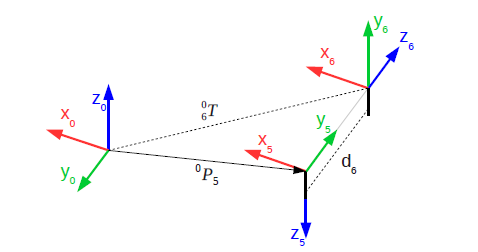
\includegraphics[height=4cm]{formulas2/1}}}
    \caption{\label{fig:formula21}}
\end{figure}
\begin{equation}
P_5^0 = P_6^0 - d_6 . \hat{Z}_6^0
\end{equation}
برای محاسبه $\theta_1$ ربات را از بالا مشاهده میکنیم:
\begin{figure}[H]%
	\centering
    \subfloat{{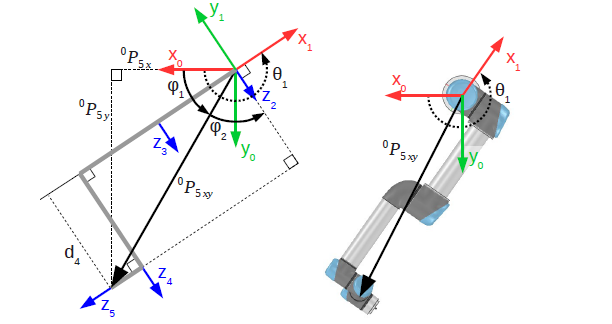
\includegraphics[height=6cm]{formulas2/3}}}
    \caption{\label{fig:formula22}}
\end{figure}
\noindent
با توجه به تصویر میبینیم که دو جوینت $0,1$ روی یکدیگر قرار دارند. زاویه $\theta_1$ با زاویه بین $x_0$ به $x_1$ در راستای $z_1$ برابر است . حال با توجه به تصویر میبینم که :
\begin{equation}
\theta_1 = \phi_1 + \phi_2 + \frac{\pi}{2}
\end{equation}
که در اینجا برای محاسبه $\phi_1$ ابتدا بردار $\overrightarrow{P50}$ را تجزیه کرده و $atan2$  میگیریم.سپس برای محاسبه  $\phi_2$ با توجه به شکل داریم:
\begin{figure}[H]%
	\centering
    \subfloat{{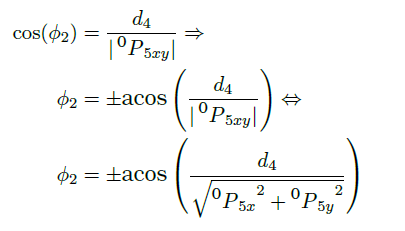
\includegraphics[height=4cm]{formulas2/5}}}
    \caption{\label{fig:formula23}}
\end{figure}
\noindent
درنهایت $\theta_1$ را با جایگذاری موارد بالا به دست می‌آوریم و داریم:
\begin{figure}[H]%
	\centering
    \subfloat{{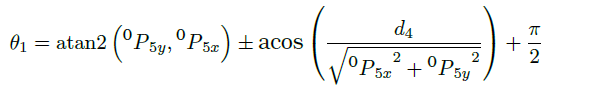
\includegraphics[height=1.5cm]{formulas2/6}}}
    \caption{\label{fig:formula24}}
\end{figure}

\subsection{محاسبه‌ی $\theta_5$}
با توجه به شکل:
\begin{figure}[H]%
	\centering
    \subfloat{{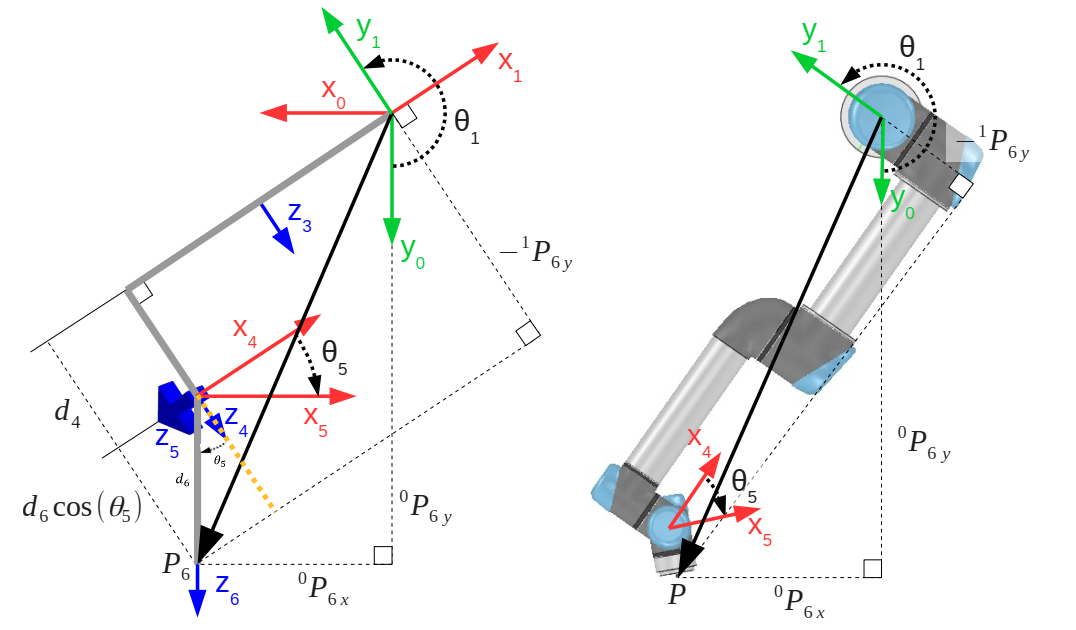
\includegraphics[height=6cm]{formulas2/7}}}
    \caption{\label{fig:formula25}}
\end{figure}
\noindent
به دو روش مختلف ${P_6^1}_y$ را محاسبه میکنیم:

\subsubsection{}
با توجه به اینکه $\theta_5$ زاویه بین $x_4$ به $x_5$ در جهت $z_5$ می‌باشد و $d_6$ برابر فاصله $x_5$  به $x_6$ در جهت $z_6$ میباشد داریم:
\begin{equation}
-P_{6y}^1 = d_4 = d_{6}cos \theta_5
\end{equation}

\subsubsection{}
روش دیگر به این صورت است که میتوان با استفاده از ترانهاده‌ی ماتریس $P_6^0$، $R_1^0$ را  را به $P_6^1$ تبدیل کرد.($P_6^0$ را از قبل داریم که در واقع موقعیت مجری نهایی نسبت به صفر هست که در ورودی داده شده است)
\begin{figure}[H]%
	\centering
    \subfloat{{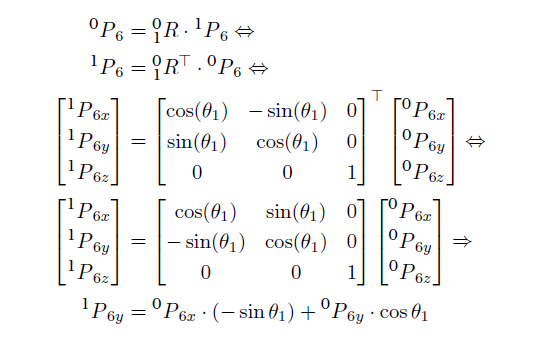
\includegraphics[height=6cm]{formulas2/9}}}
    \caption{\label{fig:formula26}}
\end{figure}
\noindent
پس این دو رابطه باهم برابر قرار میدهیم و $cos \theta_5$ را جدا میکنیم و در اخر $acos$ می‌گیریم.
\begin{figure}[H]%
	\centering
    \subfloat{{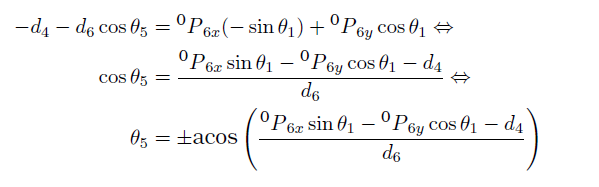
\includegraphics[height=3cm]{formulas2/10}}}
    \caption{\label{fig:formula28}}
\end{figure}
\noindent
علت $real$  گرفتن از $\theta_5$ این است که در برخی موارد مقادیر موهومی به دست می‌آیند که مدنظر ما نیستند.


\subsection{محاسبه‌ی $\theta_6$}
به دو روش $\theta_6$ را به دست می‌آوریم:
\subsubsection{}
ماتریس $R_0^1$  و $R_6^0$  را داریم این دو را در یک دیگر ضرب میکنیم سپس ستون دوم ماتریس دوران را برداشته و به نام $Y_1^6$ قرار میدهیم که برحسب $\theta_1$ خواهد بود که ما  $\theta_1$ را از مرحله قبل به دست اوردیم. داریم:
\begin{figure}[H]%
	\centering
    \subfloat{{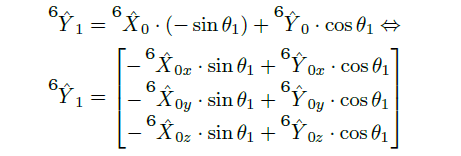
\includegraphics[height=2.5cm]{formulas2/11}}}
    \caption{\label{fig:formula29}}
\end{figure}

\subsubsection{}
با توجه به شکل زیر:
\begin{figure}[H]%
	\centering
    \subfloat{{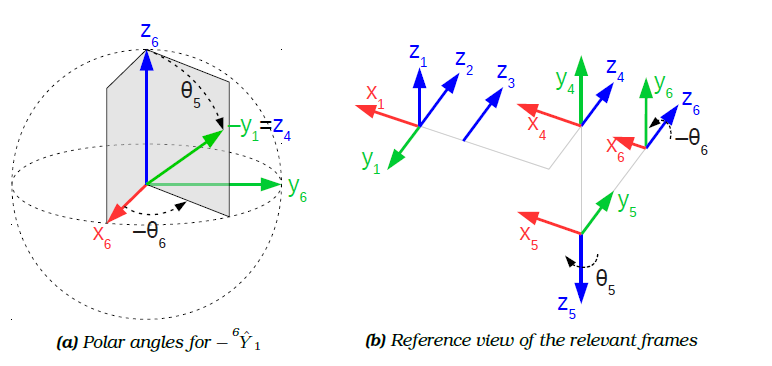
\includegraphics[height=5cm]{formulas2/12}}}
    \caption{\label{fig:formula210}}
\end{figure}
\noindent
و تبدیل مختصات کروی به کارتزین و روابط زیر:
\begin{figure}[H]%
	\centering
    \subfloat{{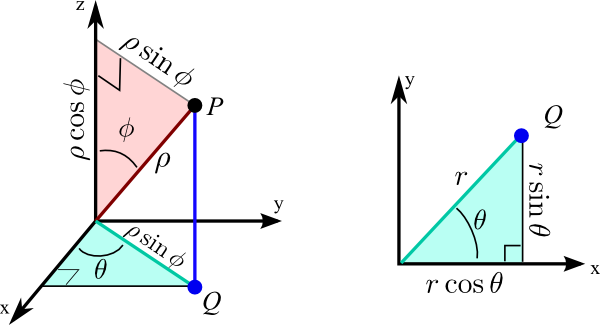
\includegraphics[height=3.5cm]{formulas2/13}}}
    \\
    \subfloat{{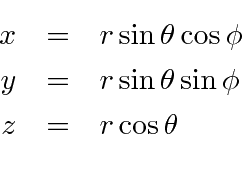
\includegraphics[height=2.5cm]{formulas2/14}}}
    \caption{\label{fig:formula211}}
\end{figure}
\noindent
داریم:
\begin{figure}[H]%
	\centering
    \subfloat{{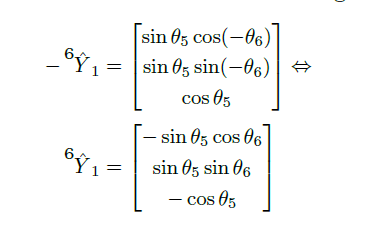
\includegraphics[height=3.5cm]{formulas2/15}}}
    \caption{\label{fig:formula212}}
\end{figure}
\noindent
این دو رابطه را باهم برابر قرار میدهیم و به نتایج زیر میرسیم:
\begin{figure}[H]%
	\centering
    \subfloat{{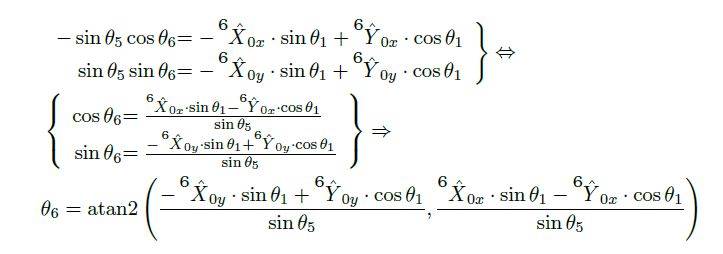
\includegraphics[height=4cm]{formulas2/162}}}
    \caption{\label{fig:formula213}}
\end{figure}
\noindent
و چون در مخرج $sin \theta_5$ داریم یک شرط میگذاریم که در صورتی که سینوس صفر شود یک مقدار رندم دیگر به $\theta_6$ میدهیم.


\subsection{محاسبه‌ی $\theta_3$}
ابتدا تابع $DH$ را فراخوانی میکنیم.(دقت شود مقادیر به دست امده برای $\theta_1, \theta_5, \theta_6$ را نیز به عنوان ورودی میدهیم)
با استفاده از ماتریس های $T$، $T_4^1$ را به دست می اوریم سپس ستون اخر آن را که همان $P_4^1$ است درایه $x, z$ را برداشته و اندازه $P_{4_{xz}}$ را به دست  می‌آوریم.
\begin{figure}[H]%
	\centering
    \subfloat{{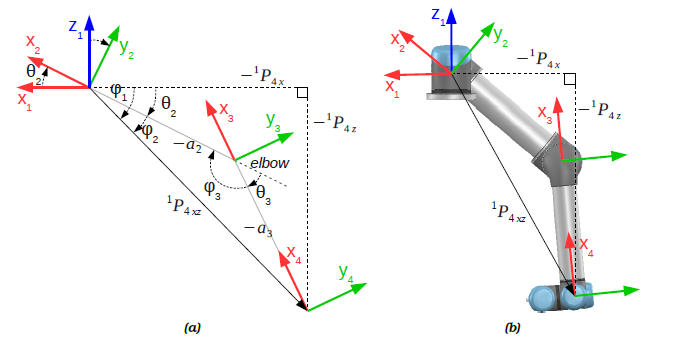
\includegraphics[height=6cm]{formulas2/16}}}
    \caption{\label{fig:formula216}}
\end{figure}
\noindent
با توجه به شکل میبینیم که $\theta_3$  مکمل $\phi_3$ میباشد.میتوان $\phi_3$ را با استفاده از قضیه $cos$ ها به دست آورد. داریم:
\begin{figure}[H]%
	\centering
    \subfloat{{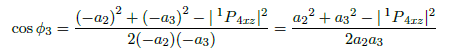
\includegraphics[height=1cm]{formulas2/17}}}
    \\
    \subfloat{{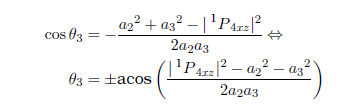
\includegraphics[height=1.5cm]{formulas2/192}}}
    \\
    \subfloat{{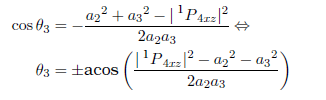
\includegraphics[height=2cm]{formulas2/18}}}
    \caption{\label{fig:formula220}}
\end{figure}
\subsection{محاسبه‌ی $\theta_2$}
با توجه به شکل \ref{fig:formula216} داریم:
\begin{equation}
\theta_2 = \phi_1 - \phi_2
\end{equation}
که $\phi_1$ را با استفاده از ${P_4^1}_z, {P_4^1}_x$ و $atan2$ به دست می اوریم.($P$ ها نیز از روی ماتریس $T_1^4$ به دست امده اند)
برای محاسبه $\phi_2$ نیز از قضیه سینوس ها استفاده میکنیم و ${P_4^1}_{xz}$ را نیز از مرحله قبل داریم.
درنتیجه:
\begin{figure}[H]%
	\centering
    \subfloat{{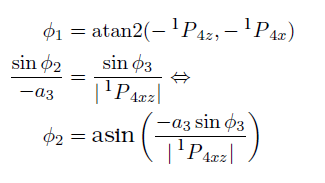
\includegraphics[height=4cm]{formulas2/19}}}
    \qquad
    \subfloat{{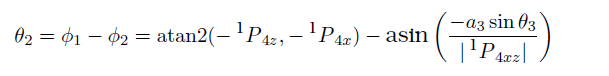
\includegraphics[height=1.5cm]{formulas2/20}}}
    \caption{\label{fig:formula221}}
\end{figure}
\noindent
\subsection{محاسبه‌ی $\theta_4$}
ابتدا تابع $DH$ را فراخوانی میکنیم.(دقت شود مقادیر به دست امده برای $\theta_{1,2,3,5,6}$ را نیز به عنوان ورودی میدهیم)
 با استفاده از $T$ ها $T_3^4$ را محاسبه میکنیم:
\begin{figure}[H]%
	\centering
    \subfloat{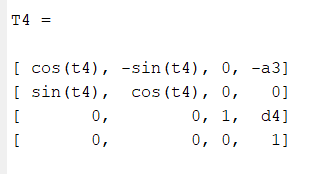
\includegraphics[height=4cm]{formulas2/21}}
    \caption{\label{fig:formula222}}
\end{figure}
\noindent
باتوجه به این ماتریس درایه $2,1$ ستون اول را برداشته و $atan2$ میگیریم تا $\theta_4$ به دست اید.
سپس $q$ ها را باهم \lr{concatenate} میکنیم و به صورت بردار $\overrightarrow{Q}$ خروجی میدهیم.
در بخش  \lr{inverse Kinematic} تابع \lr{inverse} را با ورودی های موقعیت و جهت گیری مجری نهایی فراخوانی میکنیم.

\subsection{صحت‌سنجی سینماتیک معکوس}
برای راستی ازمایی یک \lr{path} درست کرده ایم که $q_1$ از $-90$ تا $90$  درجه میرود.
یک حلقه از  $-0.5$ تا $0.5$ تعریف میکنیم با گام های $0.1$ که هر بار $t$ که بردار متغیر های مفصلی ما هست همه را صفر قرار میدهیم ولی مقدار $t(1)$ را  $i\times\pi$ می‌گذاریم. سپس تابع $DH$ را با $t$ و بقیه پارامتر های$a, d$ فراخوانی میکنیم و $P, R$ را از دل ماتریس $T$ بیرون میکشیم.
با توجه به ماتریس شکل \ref{fig:formula223} مقادیر $\alpha, \beta, \gamma$ را به دست می اوریم و به تابع \lr{inverse}  میدهیم و $Q$ را به دست می اوریم.
\\
\begin{figure}[H]%
	\centering
    \subfloat{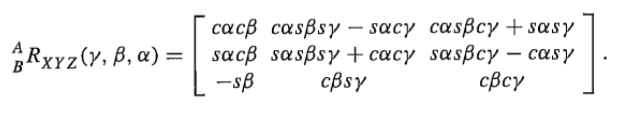
\includegraphics[height=2cm]{formulas2/22}}
    \caption{\label{fig:formula223}}
\end{figure}
\noindent
سپس \lr{Link} های ربات را تعریف کرده و با \lr{serialLink} انها را به هم متصل میکنیم. در نهایت $ur.plot$  میکنیم که ورودی را نیز $Q$ میدهیم($Q$ هر بار که حلقه طی میشود تغییر میکند.)
در میبینیم که مفصل اول یک نیم دایره را طی میکند که البته لزوما $Q$ هایی که به ما میدهد ان چیزی نیست که ما فکر میکنیم چون به هر نقطه در فضای کاری میتوان با چند جهت گیری رسید.مهم این است که مسیر مورد نظر مارا طی میکند.



\section{به دست آوردن ماتریس ژاکوبین}
ما دونوع ژاکوبین داریم: 1. \lr{velocity propagation} 2. \lr{general}
\subsection{ژاکوبین \lr{general}}
در ژاکوبین \lr{general}  ما به ردیف 1 تا 3 ستون سوم و ستون اخر ماتریس $T$ نیاز داشتیم که ردیف 1تا 3 ستون سوم $z$ و ردیف آخر $o$ نامگذاری شده است.
با توجه به  \lr{modified} بودن نامگذاری محور‌ها و نوع  \lr{joint} ها که همگی  \lr{revolute} هستند از رابطه‌ی \ref{eq:eq1} استفاده می‌کنیم.
\\
یک تابع با نام \lr{Jacobain\_General} تعریف کرده‌ایم که خروجی آن یک ماتریس  $6\times6$ می‌باشد که سه ردیف بالا مربوط به ژاکوبین خطی است و سه ردیف اخر مربوط به ژاکوبین زاویه‌ای می‌باشد و ورودی آن هم $t$  هست تا اگر خواستیم به $t$ ها مقدار دهیم ($t$ در واقع زاویه های هر \lr{joint} می‌باشد).
به پارامتر های $a, d$ مقدار داده‌ایم(اگرچه میتوان این تابع را به صورت سیمبولیک هم اجرا کرد).
\\
در ابتدا یک بار $DH$ و $RDH$ را فراخوانی می‌کنیم سپس خروجی این دو تابع را با دستور $cat$ پشت سر هم قرار می دهیم در واقع ماتریس‌های $R$ و $T$ به دست آمده را به صورت مجزا پشت سر هم قرار می‌دهیم و یک ارایه 3 بعدی می‌سازیم.
\\
حلقه‌ی مربوط به $o$ هم برای به دست اوردن ماتریس $T_{ee}$ نسبت به $frame_{0}$ است تابتوانیم از ردیف 1 تا 3 ستون اخر آن در محاسبه  ژاکوبین‌ها استفاده کنیم.
یک حلقه 6 تایی می‌نویسیم، هر بار طی شدن حلقه مربوط به یک  \lr{joint} می‌باشد. درون این حلقه دو ماتریس \lr{T\_current} و \lr{R\_current}  را به صورت همانی تعریف می‌کنیم. حال با نوشتن یک حلقه دیگر از 1 تا $i$ (شماره‌ی \lr{joint} مربوطه) $T_{i}$ و $R_{i}$ را نسبت به $frame_{0}$ حساب می‌کنیم. باتوجه به روابط مربوط به جزوه، ستون $i$ ماتریس $j_{\omega}$ و $j_{v}$ را حساب می‌کنیم. (دقت شود با هر بار طی شدن حلقه‌ی اصلی ماتریس‌های \lr{T\_current} و \lr{R\_current}  دوباره تبدیل به ماتریس همانی می‌شوند)
در قسمت   \lr{Jacobian-General}،  ابتدا $t$ را که ورودی تابع است به صورت $syms$ و یک بردار ردیفی 6 تایی تعریف می‌کنیم و  تابع ژاکوبین را فراخوانی میکنیم سپس $j_{\omega}$ و $j_{v}$ به دست آمده را \lr{simplify} کرده و سپس \lr{concatanate} می‌کنیم.

%\begin{equation}
%J_{6 \times 6} = \begin{bmatrix}
%J_{v} \\
%J_{\omega}
%\end{bmatrix}
%\quad
%J_{v} = J_{\omega a} \\
%J_{\omega_{3 \times 6}} = [z_{0}^{0} | R_{1}^{0} Z_{1}^{1} | R_{2}^{0} Z_{2}^{2} | %R_{3}^{0} Z_{3}^{3} | R_{4}^{0} Z_{4}^{4} | R_{5}^{0} Z_{5}^{5} | R_{6}^{0} Z_{6}^{6}]
%\label{eq:eq1}
%\end{equation}

\subsection{ژاکوبین \lr{velocity-omega}}
در این روش ابتدا باید $v$ و $\omega$ را به دست آوریم در نتیجه یک تابع با نام \lr{velocity\_omega} تعریف کرده ایم که در ابتدا $v$ و $\omega$ را برابر یک بردار سه تایی 0 قرار می‌دهیم. $t$ و $q$ را به صورت متغیر های سمبولیک و یک بردار افقی 6 تایی تعریف می‌کنیم و به $a, d$ ها هم مقدار داده‌ایم.
سپس دوباره توابع \lr{DH, RDH} را فراخوانی می‌کنیم و $T$ها و $R$ها را باهم  \lr{cat} می‌کنیم تا به صورت یک ماتریس سه بعدی در بیایند.
\\
سپس یک حلقه ی 6 تایی مینویسم و در آن ماتریس $P$ را برابر ماتریس $T_{i+1}$ نسبت به $frame_{i}$ قرار می‌دهیم زیرا بعدا به ردیف 1تا 3  ستون آخر آن نیاز داریم.
\\
با توجه به اینکه محور ها \lr{Modified} هستند و مفصل‌ها \lr{revolute} هستند، از روابط \ref{eq:eq2} استفاده کرده و در حلقه ی  مربوطه $v$ و $\omega$  نهایی را حساب میکنیم. چون $v$ و $\omega$ که هر بار به دست می اوریم نسبت به همان \lr{frame} میباشد درنتیجه $v$ و $\omega$ نهایی نسبت به$ frame_{ee}$ می‌باشند. در نتیجه در ماتریس $RT$ ضرب میکنیم تا نسبت به $frame_{0}$ آن را به دست آوریم.(دقت شود هر بار در $v$ و $\omega$ از $v$ و $\omega$ قبلی استفاده می‌شود و هر بار اپدیت هم می‌شوند)
\begin{equation}
\begin{gathered}
\prescript{i+1}{}{\omega_{i+1}} = \prescript{i+1}{i}{R} \prescript{i}{}{\omega_i} + \dot{\theta}_{i+1} \prescript{i+1}{}{\hat{Z}_{i+1}} \\
\prescript{i+1}{}{v_{i+1}} = \prescript{i+1}{i}{R}(\prescript{i}{}{v_i}+\prescript{i}{}{\omega _i} \times \prescript{i}{}{P_{i+1}})
\end{gathered}
\label{eq:eq2}
\end{equation}
در روش اصلی، باید اینگونه باشد که یک ماتریس به دست اوریم که باضرب در یک بردار ستونی که شامل مشتق متغیر های مفصل میباشد به $v$ و $\omega$ نهایی برسیم که ماتریس های به دست امده $j_{v}$ و $j_{\omega}$  خواهند بود.
\\
ایده ای که در اینجا پیاده سازی شده بدین گونه است که ما به جای استفاده از  مشتق $t$ ها یک بردار سیمبولیک با نام $q$ تعریف کرده ایم  و درنتیجه برای مثال اگر از درایه اول $v$ نسبت به $q(1)$ مشتق بگیریم بقیه $q$ ها صفر می‌شوند و ضرایبشان از بین میرود در نتیجه ضریب $q(1)$ باقی می‌ماند و در درایه 11 ماتریس $j_{v}$ قرار می‌گیرد.
\\
با یک حلقه 6 تایی این کار انجام شده است و نتایج مربوط به $j_{\omega}$  و نتایج مربوط به $j_{v}$ را باهم   \lr{concatenate} می‌کنیم تا $j_{v}$ و $j_{\omega}$ به دست بیایند.
\\
حال در بخش مربوط به  \lr{Jacobian\_Velocity\_propagation} تابع \lr{velocity\_omega} را فراخوانی کرده و تابع  \lr{Jacobain\_Velocity\_propagation} را با خروجی تابع قبلی فراخوانی میکنیم.
سپس با \lr{concatenate} کردن $j_{v}$ و $j_{\omega}$ به دست آمده، به ژاکوبین اصلی می‌رسیم.

\section{به دست آوردن تکینگی‌های ربات}
در ابتدا \lr{serial Link} ها را تعریف کرده ایم. حال یک حلقه ی 6 تایی داریم که متغیر های مفصلی را با گام‌های$0.2, 0.2$ جلو میبرد و سپس ژاکوبین  \lr{general} را با متغیر های مفصلی حلقه ها فراخوانی میکنیم و $j_{v}$ و $j_{\omega}$ را \lr{concatenate} می‌کنیم.
\\
سپس دترمینان ژاکوبین را حساب کرده و اگر از یک حد مشخصی کمتر بود آن حالت را $ur.plot$ می‌کنیم. همه ی حالت های  \lr{singular} را با گام های $ 0.001$ ثانیه ای $ur.plot$ می‌کنیم.
\\
روش دیگر(همان قسمت کامنت شده) در این روش سه مفصل اخر را در یک  جهت گیری قفل کرده ایم که این جهت گیری موجب  \lr{singularity} نمی‌شود و سه جوینت اول را مچرخانیم چون در روش قبلی زمان زیادی طول میکشد تا کشیدگی ها را رد کند و به نقاط واضح تر  \lr{singularity} برسد.
\\
در این روش سه لینک اخر را بدون \lr{offset} در نظر میگیریم و ماتریس ژاکوبین را به صورت بلوکی یعنی 4 ماتریس $3\times3$ می‌نویسیم که شامل $ J11,J12,J22,J21 $ می‌شود. $J11$ مربوط به سه لینک اول و ژاکوبین خطی انهاست و $J21$ مربوط به سه مفصل اول و ژاکوبین زاویه ای ان ها است. $J22$ مربوط به ژاکوبین زاویه سه مفصل اخر میباشد. $J12$ صفر میشود که در واقع ژاکوبین خطی سه مفصل اخر می‌باشد که چون \lr{offset} ندارند $R$ هم ندارند که $R$ ضرب خارجی اش در $\omega$ را بتوان حساب کرد درواقع صفر می‌شود در نتیجه ماتریس ژاکوبین ما یک ماتریس پایین مثلثی میشود که در صورتی دترمینانش صفر است که دترمینان بلوک های روی قطرش صفر شود .دترمینان $J22$ صفر نمیشود چون در حالتی فیکس شده است که باعث  \lr{singularity} نشود. در نتیجه $J11$ را حساب میکنیم و اگر از حدی کوچک تر بود آن حالت را به عنوان  \lr{singularity} وارد ماتریس \lr{singular} می‌کنیم و همچنین آن ها را هم $ur.plot$ می‌کنیم.

\section{به دست آوردن دینامیک ربات}
برای محاسبه دینامیک یک تابع تعریف می‌کنیم که ورودی نمی‌گیرد و ماتریس های $D$ و $C$ و $G$ را خروجی می‌دهد و در نهایت با صدا زدن این تابع ماتریس‌های فوق محاسبه می‌شوند.
روند کلی این تابع به این صورت است که در ابتدا پارامتر های ثابت ربات، متغیر‌های مفصلی ($t$)، متغیر‌های مربوط به جرم لینک‌ها ($m$) و متغیر‌های اینرسی لینک‌ها را به طور کلی تعریف می‌کنیم و سپس با استفاده از حلقه برای هر کدام از لینک‌ها ماتریس متقارن $3\times3$ اینرسی و ماتریس سطری جرم (شامل جرم های هر لینک) را به دست می‌آوریم.
\\
سپس ماتریس‌های $D$ و $C$ و $G$ و بردار  $\overrightarrow{r_c}$ (فواصل مراکز جرم از زمین) و $P$ و همچنین برای ژاکوبین ها، ماتریس‌های $j_{v}$ و $j_{\omega}$ را با توجه به ابعادشان تعریف کرده و مقدار اولیه صفر می‌دهیم. چون در ادامه همه محاسبات به صورت سمبولیک انجام می شود، این مقداردهی اولیه را نیز با $sym$ تعریف می‌کنیم.
\\
در این بخش علاوه بر توابع $DH$ و $RDH$ که ماتریس‌های تبدیل و دوران را تولید می کردند، به تابع $DHC$ نیز نیاز داریم تا با گرفتن پارامتر های ثابت ربات، ماتریس های تبدیل مرتبط با مرکز جرم هر لینک نسبت به همان لینک را تولید کند (نسبت به پایه نیستند)، به همین ترتیب این ماتریس‌ها دوران ندارند و ماتریس دوران آن‌ها همانی است و فقط آفست‌های آن‌ها در ماتریس \lr{position} تعیین شده است.
حال پس از فراخوانی این سه تابع و با دستور $cat$، ماتریس‌ها را در یک آرایه سه بعدی پشت سر هم قرار می‌دهیم.
\\
می دانیم برای به دست آوردن $J_{vc_i}$ برای هر مفصل، در هر مرحله با تغییر مفصل و مرکز جرم، روابط مربوط به مفاصل قبل تغییر می کنند اما مفاصل بعدی آن تأثیری ندارند و ستون های مفاصل بعدی صفر می شوند. برای $J_{\omega c_i}$ نیز مفاصل بعدی بی‌تأثیر خواهند بود.
\\
به عنوان نمونه برای سه مفصل اول به این صورت خواهد بود (همه مفاصل ربات گردشی هستند):
\\
\begin{gather*}
J_{vc_{1}} = [Z_{c_{1}}^{0} \times (O_{c_{1}}^{0} - O_{1}^{0})|0|0|0|0|0] \\
J_{vc_{2}} = [Z_{c_{1}}^{0} \times (O_{c_{2}}^{0} - O_{1}^{0})|Z_{c_{2}}^{0} \times (O_{c_{2}}^{0} - O_{2}^{0})|0|0|0|0] \\
J_{vc_{3}} = [Z_{c_{1}}^{0} \times (O_{c_{2}}^{0} - O_{1}^{0})|Z_{c_{2}}^{0} \times (O_{c_{2}}^{0} - O_{2}^{0})|Z_{c_{3}}^{0} \times (O_{c_{3}}^{0} - O_{3}^{0})|0|0|0] \\
\\
J_{\omega c_{1}} = [Z_{c_{1}}^0|0|0|0|0|0]\\
J_{\omega c_{2}} = [Z_{c_{1}}^0|Z_{c_{2}}^0|0|0|0|0]\\
J_{\omega c_{3}} = [Z_{c_{1}}^0|Z_{c_{2}}^0|Z_{c_{3}}^0|0|0|0]\\
\end{gather*}
\\
بنابراین در هر مرحله برای محاسبه $J_{vc}$ به ماتریس‌های $T_c^0$ و $T_i^0$ و $R_i^0$ و ماتریس های  $T_c^0$ و $R_j^0$ که $j<i$ است نیاز داریم. به همین منظور برای محاسبه  $T_c^0$ و $T_i^0$ و  $R_i^0$ ابتدا خارج از حلقه دو ماتریس همانی $current$ تعریف می‌کنیم و در هر بار گذر حلقه ماتریس‌های  $T_{c_i}^{i-1}$ و $T_{i}^{i-1}$ و $R_{i}^{i-1}$ در ماتریس‌های مفاصل قبلی ضرب می‌شوند و در هر حلقه ماتریس‌های $T_{c_i}^0$ و $R_i^0$ را در ماتریس های $stack$ شان ذخیره می کنیم.
\\
حال با داشتن ماتریس‌های فوق و مطابق روابط بالا $J_{vc_i}$ و $J_{\omega c_i}$ برای هر مفصل محاسبه می‌شوند.
\\
در ادامه برای هر مفصل مقدار مولفه‌ی $z$ بردار $\overrightarrow{O_{c_i}^0}$ را برای $\overrightarrow{r_c}$ آن مفصل قرار می‌دهیم (فواصل مراکز جرم تا زمین) و ماتریس $D$ را نیز با توجه به رابطه‌ی آن تشکیل می‌دهیم.
\\
روابط ماتریس $D$ و $C$ و $G$ و $P$ به صورت زیر هستند:
\begin{figure}[H]%
    \centering
    \subfloat{{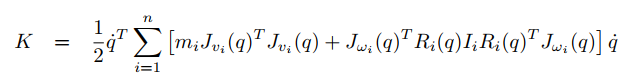
\includegraphics[height=1cm]{formulas/13}}}
    \qquad
    \subfloat{{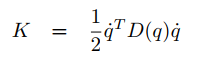
\includegraphics[height=1cm]{formulas/14}}}
    \qquad
    \subfloat{{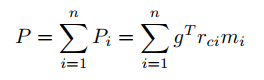
\includegraphics[height=1cm]{formulas/15}}}
    \\
    \subfloat{$G_k = \frac{\partial P}{\partial q_k}$}
    \caption{روابط ماتریس‌های دینامیکی\label{fig:formula5}}
\end{figure}
\noindent
برای ماتریس $C$ به 3 اندیس و در نتیجه 3 حلقه تو در تو نیاز داریم که در آن با توجه به فرمول $c_{ijk}$ نسبت به عناصر ماتریس $D$ مشتق گرفته و ماتریس $C$ را به صورت زیر پر 
می‌کند:
\begin{equation}
c_{ijk} := \frac{1}{2}\{\frac{\partial{d_{kj}}}{\partial{q_i}} + \frac{\partial{d_{ki}}}{\partial{q_j}} - \frac{\partial{d_{ij}}}{\partial{q_k}}\}
\end{equation}
\begin{equation}
C_k = [\sum_{j=1}^{n} c_{1jk} \sum_{j=1}^{n} c_{2jk} ... \sum_{j=1}^{n} c_{njk}]
\end{equation}
در ادامه برای استفاده بهینه از حلقه با استفاده از اندیس اول ($k$) ماتریس $P$ را نیز با توجه به رابطه‌اش تشکیل می دهیم که در آن $g$ را برابر $9.8$ قرار داده‌ایم.
در آخر نیز در یک حلقه جداگانه با مشتق گرفتن از عناصر ماتریس $P$ نسبت به متغیر مفصلی، ماتریس $G$ را محاسبه می‌کنیم.
\end{document}